\documentclass[../../main.tex]{subfiles}

\begin{document}

      \begin{figure}[H]
        \centering
        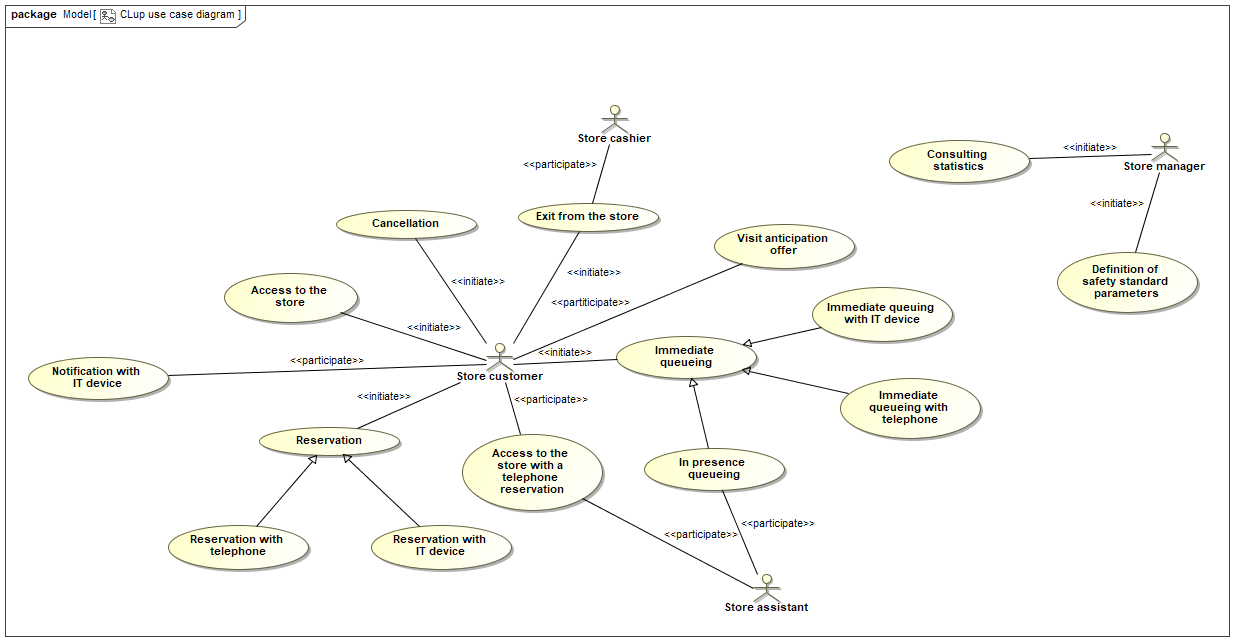
\includegraphics[width=\textwidth]{CLup_use_case_diagram.png}
        \caption{Use case diagram}
      \end{figure}

      \subsection{Immediate queueing with IT device}

      \begin{table}[H]
        \centering
          \begin{tabular}{c m{.75\textwidth}}
          \hline
          \textbf{Use Case} & Immediate queueing with IT device\\ \hline
          \textbf{Actor} & Store customer\\ \hline
          \textbf{Entry condition} & The customer wants to access a store as soon as possible\\  \hline
          \textbf{Flow of events} & \begin{itemize}
                                      \item The customer selects the store they want to access
                                      \item The customer inserts the expected duration of the visit
                                      \item The customer inserts the categories of products they want to buy
                                      \item The customer confirms their intention
                                      \item The system estimates the expected duration of the visit and the visited departments
                                      \item The system checks if the store has a free slot for the customer
                                      \item The store has a free slot
                                      \item The system queues the customer
                                    \end{itemize}\\ \hline
          \textbf{Exit condition} & The system shows a confirmation message to the user \\ \hline
          \textbf{Exceptions} &  If the store does not currently have a free time slot, the system will suggest an alternative store.
                                  
                                If the customer still wants to queue for their store of choice, the system queues the user for the first available time slot. \\ \hline
          \textbf{Mapped requirements} & R1, R6, R4, R8, R9, R13, R14, R15\\ \hline
          \end{tabular}
      \end{table}

      \begin{figure}[H]
        \centering
        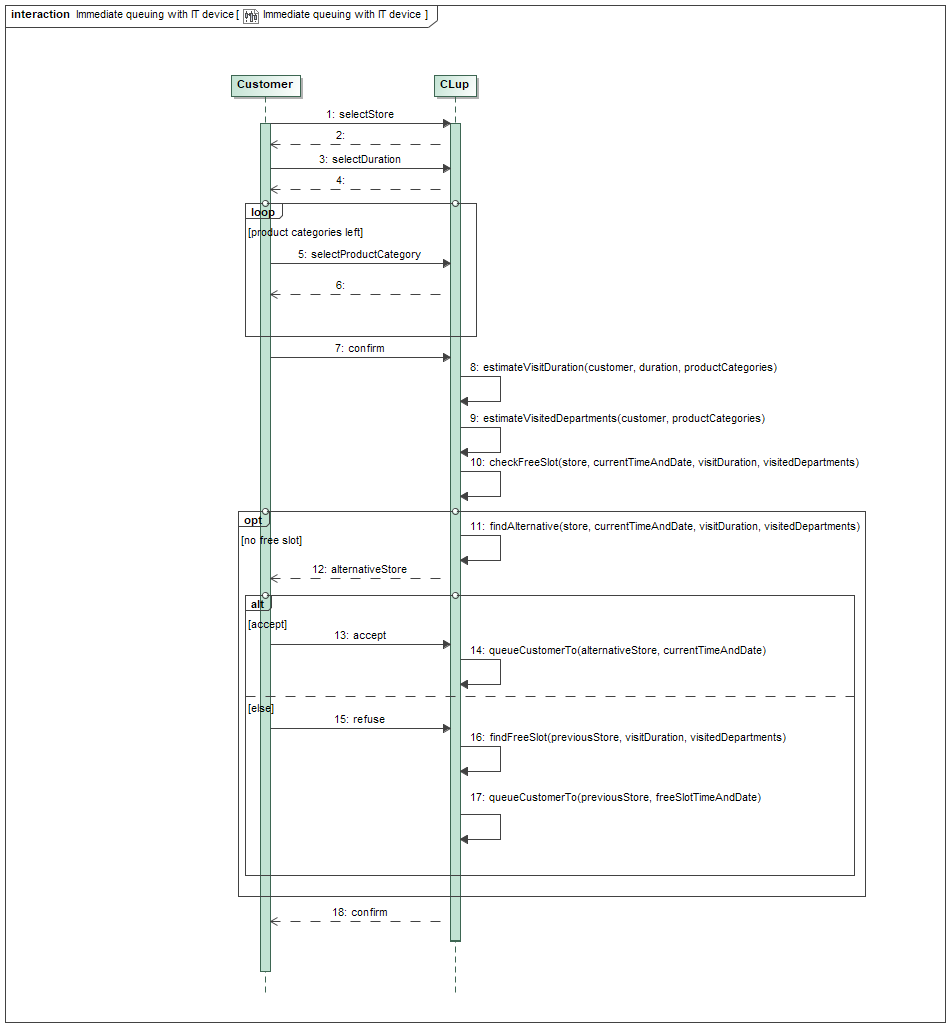
\includegraphics[width=\textwidth]{Immediate_queueing_with_IT_device.png}
        \caption{Immediate queuing with IT device sequence diagram}
      \end{figure}

      \subsection{Reservation with IT device}

      \begin{table}[H]
        \centering
          \begin{tabular}{c m{.75\textwidth}}
          \hline
          \textbf{Use Case} & Reservation with IT device\\ \hline
          \textbf{Actor} & Store customer\\ \hline
          \textbf{Entry condition} & The customer wants to reserve a visit to the store\\  \hline
          \textbf{Flow of events} & \begin{itemize}
                                      \item The customer selects the store they want to access
                                      \item The customer selects the time and date of the visit
                                      \item The customer confirms their intention
                                      \item The system estimates the expected duration of the visit and the visited departments
                                      \item The system checks if the store has a free slot for the customer
                                      \item The store has a free slot
                                      \item The system queues the customer in the time slot
                                    \end{itemize}\\ \hline
          \textbf{Exit condition} & The system shows a confirmation message to the user \\ \hline
          \textbf{Exceptions} & If the desired time slot and store are not compatible with the current scheduled queue, the system will suggest an alternative. \\ \hline
          \textbf{Mapped requirements} & R1, R6, R7, R8, R9, R13, R14, R15\\ \hline
          \end{tabular}
      \end{table}

      \begin{figure}[H]
        \centering
        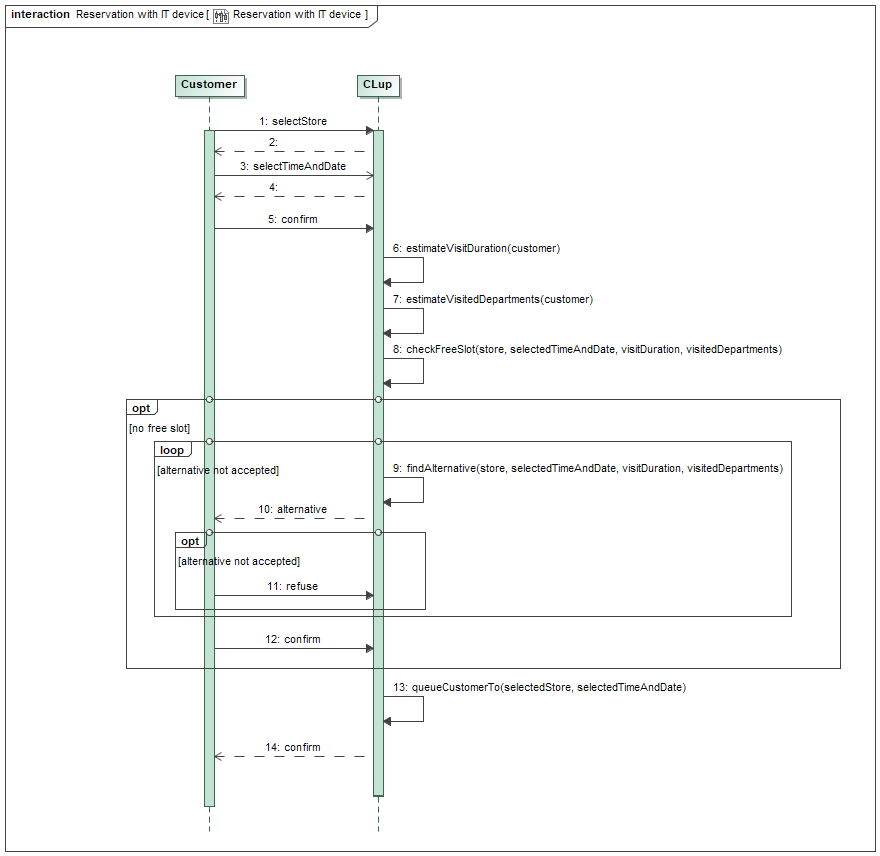
\includegraphics[width=\textwidth]{Reservation_with_IT_device.png}
        \caption{Reservation with IT device sequence diagram}
      \end{figure}


      \subsection{Cancellation}

      \begin{table}[H]
        \centering
          \begin{tabular}{c m{.75\textwidth}}
          \hline
          \textbf{Use Case} & Cancellation\\ \hline
          \textbf{Actor} & Store customer\\ \hline
          \textbf{Entry condition} & A customer wants to cancel their reservation\\  \hline
          \textbf{Flow of events} & \begin{itemize}
                                      \item The customer select the cancellation option
                                      \item CLup removes the customer from the queue
                                    \end{itemize}\\ \hline
          \textbf{Exit condition} & The system shows a confirmation message to the user \\ \hline
          \textbf{Exceptions} &\\ \hline
          \textbf{Mapped requirements} & R16\\ \hline
          \end{tabular}
      \end{table}

      \begin{figure}[H]
        \centering
        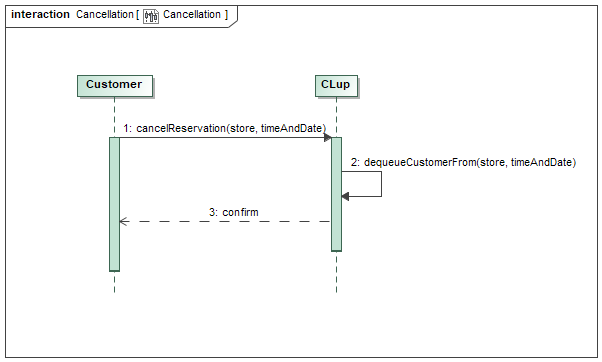
\includegraphics[width=\textwidth]{Cancellation.png}
        \caption{Cancellation sequence diagram}
      \end{figure}

      
      \subsection{Visit anticipation offer}

      \begin{table}[H]
        \centering
          \begin{tabular}{c m{.75\textwidth}}
          \hline
          \textbf{Use Case} & Visit anticipation offer\\ \hline
          \textbf{Actor} & Store customer\\ \hline
          \textbf{Entry condition} & A customer cancels their reservation\\  \hline
          \textbf{Flow of events} & \begin{itemize}
                                      \item CLup checks if there is some user wanting to access the store as soon as possible and scheduled for a later visit
                                      \item CLup sends a notification to the customer, offering to move up the visit
                                      \item The customer accepts the offer
                                      \item CLup queues the customer in the time slot
                                    \end{itemize}\\ \hline
          \textbf{Exit condition} & The system shows a confirmation message to the user \\ \hline
          \textbf{Exceptions} & If no user accepts, the slot is kept free. \\ \hline
          \textbf{Mapped requirements} & R14, R15, R16\\ \hline
          \end{tabular}
      \end{table}

      \begin{figure}[H]
        \centering
        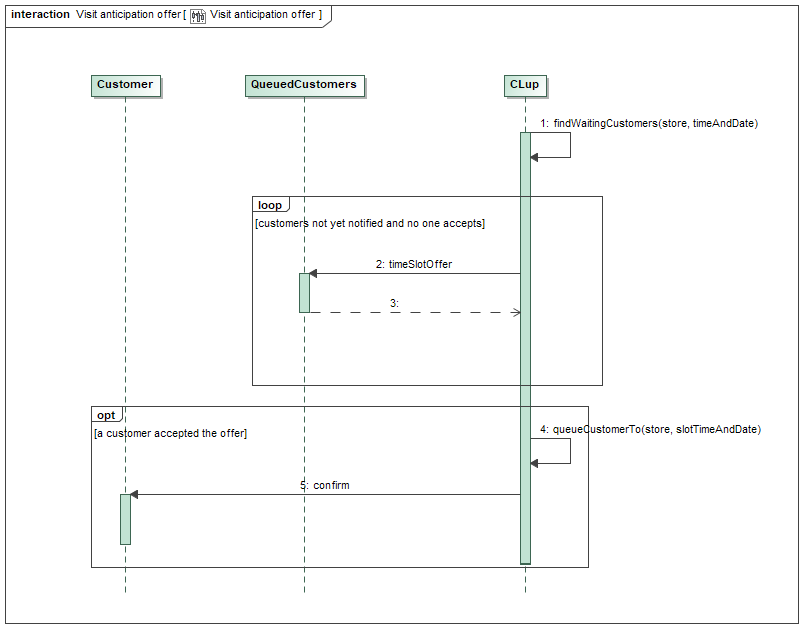
\includegraphics[width=\textwidth]{Visit_anticipation_offer.png}
        \caption{Visit anticipation offer sequence diagram}
      \end{figure}


      \subsection{Notification with IT device}

      \begin{table}[H]
        \centering
          \begin{tabular}{c m{.75\textwidth}}
          \hline
          \textbf{Use Case} & Notification with IT device \\ \hline
          \textbf{Actor} & Store customer\\ \hline
          \textbf{Entry condition} & A customer's visit start time is near\\  \hline
          \textbf{Flow of events} & \begin{itemize}
                                      \item CLup sends the customer a notification to remind them of the visit
                                    \end{itemize}\\ \hline
          \textbf{Exit condition} & The customer approaches the store \\ \hline
          \textbf{Exceptions} & \\ \hline
          \textbf{Mapped requirements} & R10, R11\\ \hline
          \end{tabular}
      \end{table}

      \begin{figure}[H]
        \centering
        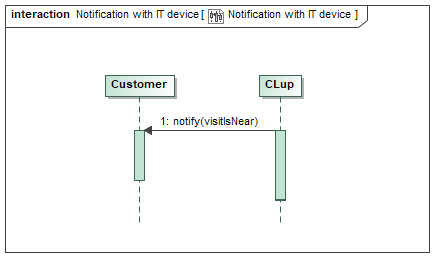
\includegraphics[width=\textwidth]{Notification_with_IT_device.png}
        \caption{Notification with IT device sequence diagram}
      \end{figure}


      \subsection{Access to the store}

      \begin{table}[H]
        \centering
          \begin{tabular}{c m{.75\textwidth}}
          \hline
          \textbf{Use Case} & Access to the store \\ \hline
          \textbf{Actor} & Store customer\\ \hline
          \textbf{Entry condition} & A customer approaches the store\\  \hline
          \textbf{Flow of events} & \begin{itemize}
                                      \item The customer scans their receipt at the store entrance
                                      \item CLup checks if the current time is compatible with the receipt's start time slot
                                    \end{itemize}\\ \hline
          \textbf{Exit condition} & CLup allows the customer to enter the store \\ \hline
          \textbf{Exceptions} & If the customer scans the receipt outside their time slot, they are not allowed to enter the store. \\ \hline
          \textbf{Mapped requirements} & R10, R12\\ \hline
          \end{tabular}
      \end{table}

      \begin{figure}[H]
        \centering
        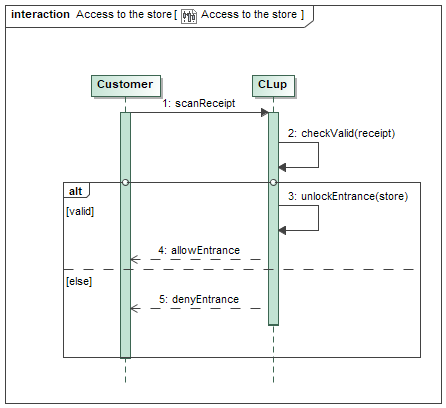
\includegraphics[width=\textwidth]{Access_to_the_store.png}
        \caption{Access to the store sequence diagram}
      \end{figure}


      \subsection{Exit from the store}

      \begin{table}[H]
        \centering
          \begin{tabular}{c m{.75\textwidth}}
          \hline
          \textbf{Use Case} & Exit from the store\\ \hline
          \textbf{Actor} & Store customer, store's cashier\\ \hline
          \textbf{Entry condition} & A customer has finished shopping\\  \hline
          \textbf{Flow of events} & \begin{itemize}
                                      \item The customer shows CLup's receipt to the store's cashier
                                      \item The store's cashier scans the receipt
                                      \item CLup registers the end of the visit
                                    \end{itemize}\\ \hline
          \textbf{Exit condition} & The system shows a confirmation message to the store's cashier \\ \hline
          \textbf{Exceptions} & \\ \hline
          \textbf{Mapped requirements} & R3, R12\\ \hline
          \end{tabular}
      \end{table}

      \begin{figure}[H]
        \centering
        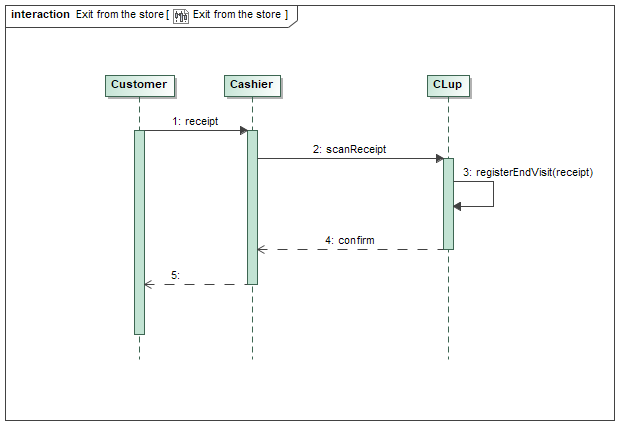
\includegraphics[width=\textwidth]{Exit_from_the_store.png}
        \caption{Exit from the store sequence diagram}
      \end{figure}


      \subsection{In presence queueing}

      \begin{table}[H]
        \centering
          \begin{tabular}{c m{.75\textwidth}}
          \hline
          \textbf{Use Case} & In presence queueing\\ \hline
          \textbf{Actor} & Store customer, store assistant\\ \hline
          \textbf{Entry condition} & A customer asks a store assistant for a line up receipt\\  \hline
          \textbf{Flow of events} & \begin{itemize}
                                      \item The store assistant accesses CLup
                                      \item The store assistant requests CLup to queue the customer
                                      \item The system estimates the expected duration of the visit and the visited departments
                                      \item The system finds the first available time slot in the assistant's store
                                      \item CLup adds the customer to the queue in the first available time slot
                                      \item CLup sends the line up receipt to the store assistant as a confirmation
                                      \item The store assistant prints the line up receipt 
                                    \end{itemize}\\ \hline
          \textbf{Exit condition} & The store assistant gives the printed line up receipt to the customer\\ \hline
          \textbf{Exceptions} & \\ \hline
          \textbf{Mapped requirements} & R1, R4, R5, R6, R8, R9\\ \hline
          \end{tabular}
      \end{table}

      \begin{figure}[H]
        \centering
        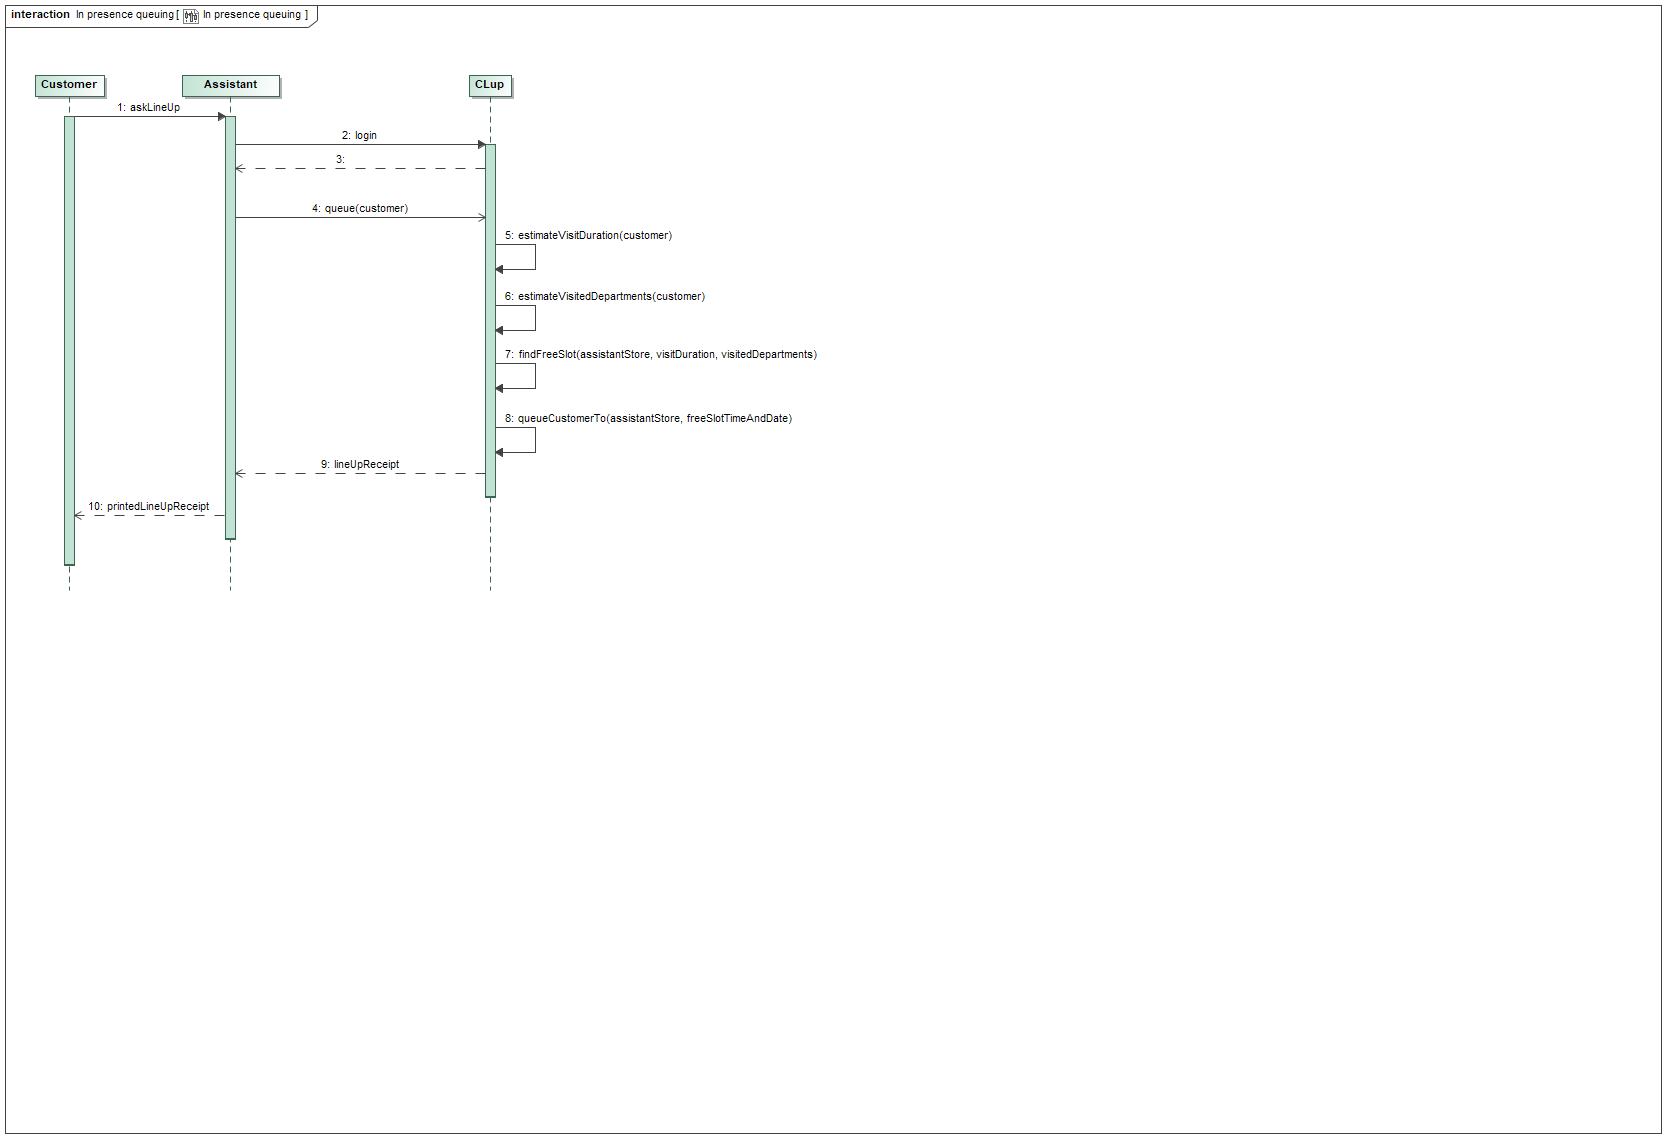
\includegraphics[width=\textwidth]{In_presence_queueing.png}
        \caption{In presence queueing sequence diagram}
      \end{figure}


      \subsection{Immediate queueing with telephone}

      \begin{table}[H]
        \centering
          \begin{tabular}{c m{.75\textwidth}}
          \hline
          \textbf{Use Case} & Queueing with telephone\\ \hline
          \textbf{Actor} & Store customer\\ \hline
          \textbf{Entry condition} & A customer calls CLup's telephone number\\  \hline
          \textbf{Flow of events} & \begin{itemize}
                                      \item CLup asks the customer if they would like to access the store as soon as possible or to reserve a time slot
                                      \item The customer says they want to access the store as soon as possible
                                      \item CLup asks which store the customer wants to access
                                      \item The customer states the store they would like to access
                                      \item CLup repeats the chosen options and asks for confirmation
                                      \item The customer confirms their intentions
                                      \item The system adds the customer to the queue to enter the store
                                      \item CLup dictates the numeric code to use at the entrance to the customer
                                      \item CLup asks for confirmation that the numeric code has been understood
                                    \end{itemize}\\ \hline
          \textbf{Exit condition} & The customer confirms \\ \hline
          \textbf{Exceptions} & If the chosen store does not have any available slot, the system suggests an alternative.
          
                                If the customer does not confirm their intentions, the system states again the available options.
                                
                                If the customer does not confirm the reception of the numeric code, the system repeats the numeric code.\\ \hline
          \textbf{Mapped requirements} & R1, R4, R8, R9, R13, R14, R15\\ \hline
                              \end{tabular}
      \end{table}

      \begin{figure}[H]
        \centering
        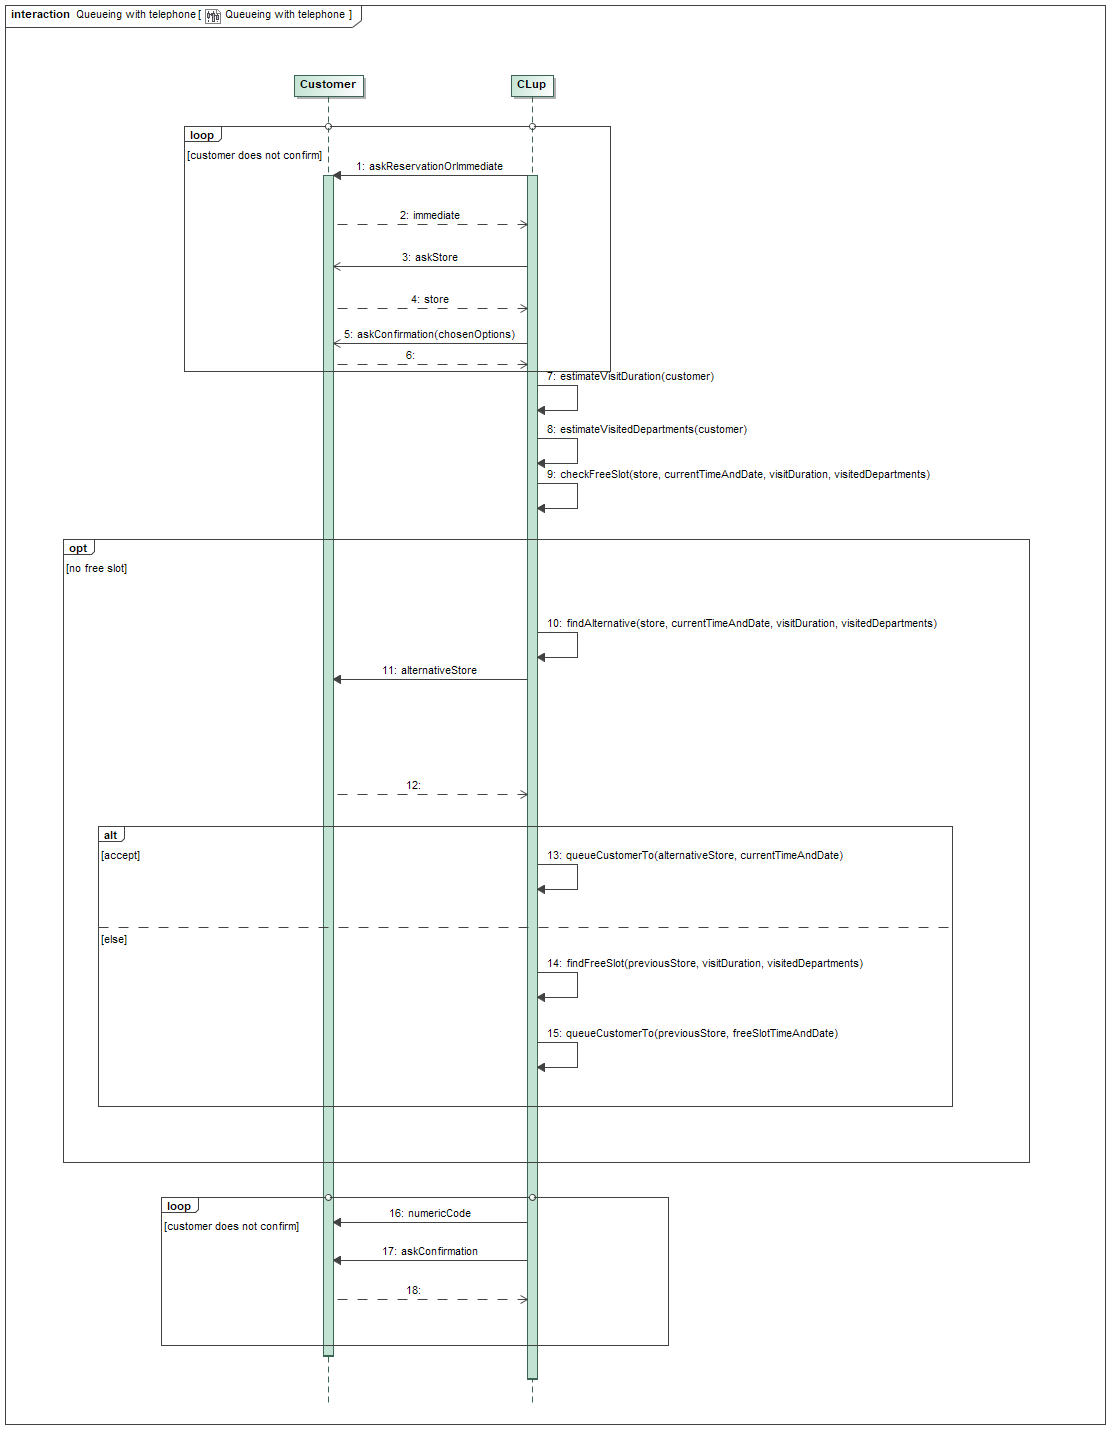
\includegraphics[width=\textwidth]{Queueing_with_telephone.png}
        \caption{Queueing with telephone sequence diagram}
      \end{figure}


      \subsection{Reservation with telephone}

      \begin{table}[H]
        \centering
          \begin{tabular}{c m{.75\textwidth}}
          \hline
          \textbf{Use Case} & Reservation with telephone\\ \hline
          \textbf{Actor} & Store customer\\ \hline
          \textbf{Entry condition} & A customer calls CLup's telephone number\\  \hline
          \textbf{Flow of events} & \begin{itemize}
                                      \item CLup asks the customer if they would like to access the store as soon as possible or to reserve a time slot
                                      \item The customer says they want to reserve a time slot
                                      \item CLup asks which store the customer wants to access
                                      \item The customer states the store they would like to access
                                      \item CLup asks in which date the customer would like to access the store
                                      \item The customer states the desired date
                                      \item CLup asks at which time the customer would like to access the store
                                      \item The customer states the desired time
                                      \item CLup repeats the chosen options and asks for confirmation
                                      \item The customer confirms their intentions
                                      \item CLup estimates the visit duration
                                      \item CLup checks if the visit is compatible with the current schedule
                                      \item The system adds the customer to the queue to enter the store
                                      \item CLup dictates the numeric code to use at the entrance to the customer
                                      \item CLup asks for confirmation that the numeric code has been understood
                                    \end{itemize}\\ \hline
          \textbf{Exit condition} & The customer confirms \\ \hline
          \textbf{Exceptions} & If the reservation is not compatible with the current schedule, the system suggests an alternative.
          
                                If the customer does not confirm their intentions, the system states again the available options.
                                
                                If the customer does not confirm the reception of the numeric code, the system repeats the numeric code.\\ \hline
          \textbf{Mapped requirements} & R1, R7, R8, R9, R13, R14, R15\\ \hline
                              \end{tabular}
      \end{table}

      \begin{figure}[H]
        \centering
        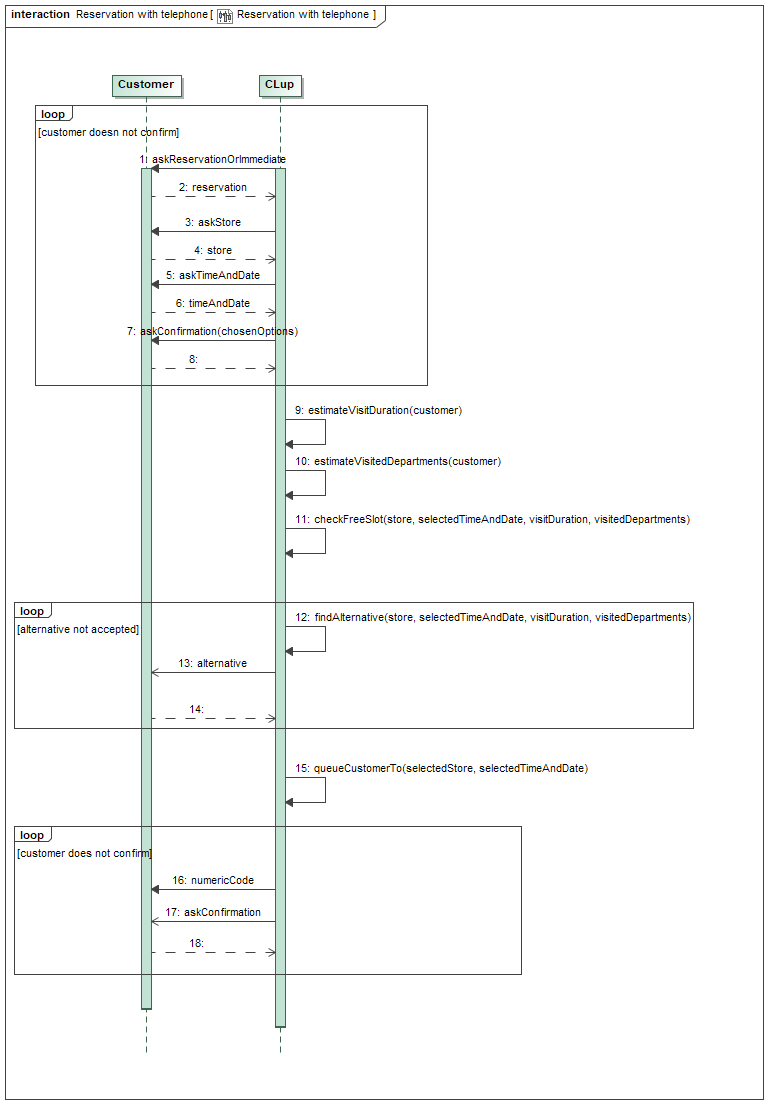
\includegraphics[width=\textwidth]{Reservation_with_telephone.png}
        \caption{Reservation with telephone sequence diagram}
      \end{figure}

      \subsection{Access to the store with a telephone reservation}

      \begin{table}[H]
        \centering
          \begin{tabular}{c m{.75\textwidth}}
          \hline
          \textbf{Use Case} & Accessing the store with a telephone reservation\\ \hline
          \textbf{Actor} & Store customer, store assistant\\ \hline
          \textbf{Entry condition} & The visit start time of a customer who has reserved a place in the queue via telephone call is near\\  \hline
          \textbf{Flow of events} & \begin{itemize}
                                      \item CLup system calls the user, to remind them of the visit
                                      \item The customer approaches the store
                                      \item The customer goes to a store assistant, and shows them the numeric code
                                      \item The store assistant accesses CLup system
                                      \item The store assistant checks the numeric code
                                    \end{itemize}\\ \hline
          \textbf{Exit condition} & The store assistant prints the line up receipt \\ \hline
          \textbf{Exceptions} & If the numeric code is invalid or expired, CLup returns an error to the store assistant.\\ \hline
          \textbf{Mapped requirements} & R6, R10, R11\\ \hline
          \end{tabular}
      \end{table}

      \begin{figure}[H]
        \centering
        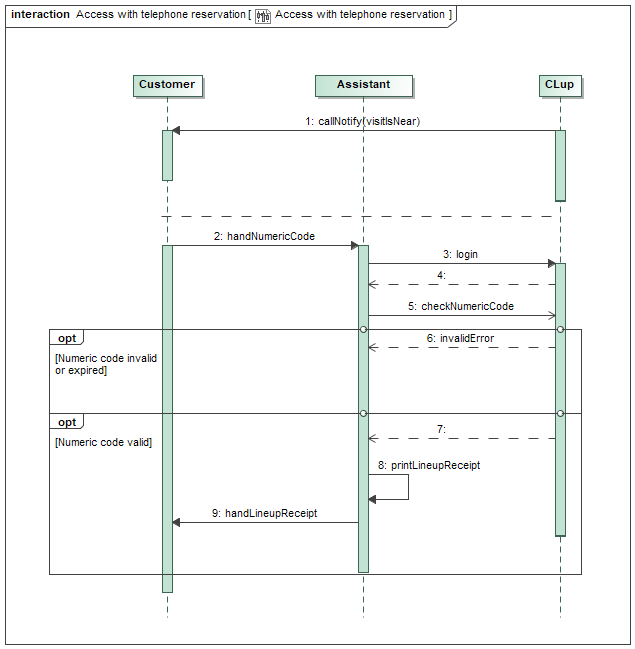
\includegraphics[width=\textwidth]{Access_with_telephone_reservation.png}
        \caption{Access with telephone reservation sequence diagram}
      \end{figure}

      \subsection{Consulting statistics}

      \begin{table}[H]
        \centering
          \begin{tabular}{c m{.75\textwidth}}
          \hline
          \textbf{Use Case} & Consulting statistics\\ \hline
          \textbf{Actor} & Store manager\\ \hline
          \textbf{Entry condition} & The store manager wants to consult current statistics\\  \hline
          \textbf{Flow of events} & \begin{itemize}
                                      \item The store manager accesses CLup
                                      \item The store manager requests current statistics to CLup
                                      \item CLup computes the requested statistics
                                    \end{itemize}\\ \hline
          \textbf{Exit condition} & CLup returns the requested statistics \\ \hline
          \textbf{Exceptions} & \\ \hline
          \textbf{Mapped requirements} & R3\\ \hline
          \end{tabular}
      \end{table}

      \begin{figure}[H]
        \centering
        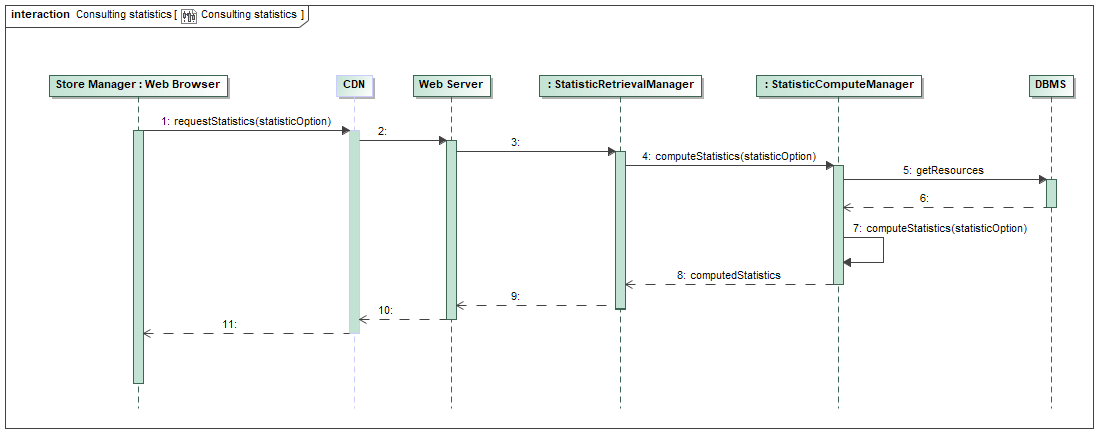
\includegraphics[width=\textwidth]{Consulting_statistics.png}
        \caption{Consulting statistics sequence diagram}
      \end{figure}

      \subsection{Definition of safety standard parameters}

      \begin{table}[H]
        \centering
          \begin{tabular}{c m{.75\textwidth}}
          \hline
          \textbf{Use Case} & Definition of safety standard parameters\\ \hline
          \textbf{Actor} & Store manager\\ \hline
          \textbf{Entry condition} & The store manager needs to define or update safety parameters \\  \hline
          \textbf{Flow of events} & \begin{itemize}
                                      \item The store manager accesses CLup
                                      \item The store manager defines or updates the needed safety parameters
                                      \item CLup asks for confirmation of the new safety parameters
                                      \item The store manager confirms
                                      \item CLup saves the new safety parameters
                                      \item CLup updates the queue availability for the store according to the newly defined safety parameters
                                    \end{itemize}\\ \hline
          \textbf{Exit condition} & CLup confirms the succeeding of the operation \\ \hline
          \textbf{Exceptions} & If the store manager does not confirm, nothing happens on CLup system, and the old safety parameters are kept.\\ \hline
          \textbf{Mapped requirements} & R2\\ \hline
          \end{tabular}
      \end{table}

      \begin{figure}[H]
        \centering
        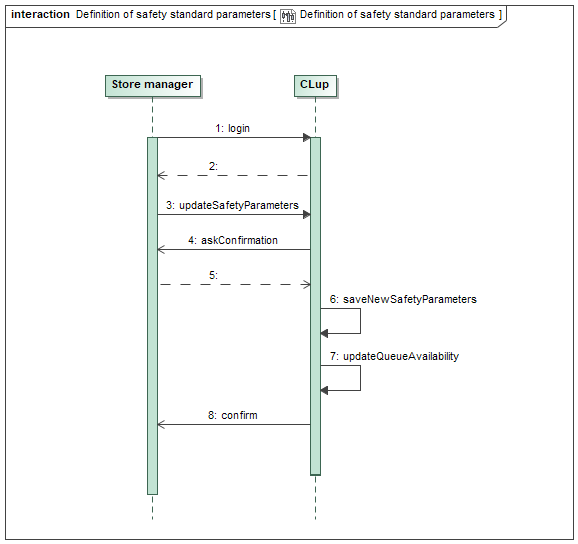
\includegraphics[width=\textwidth]{Definition_of_safety_standard_parameters.png}
        \caption{Definition of safety standard parameters sequence diagram}
      \end{figure}

\end{document}
